\documentclass[tikz,border=6pt]{standalone}
\usepackage{ifthen}
\usetikzlibrary{calc}

\begin{document}
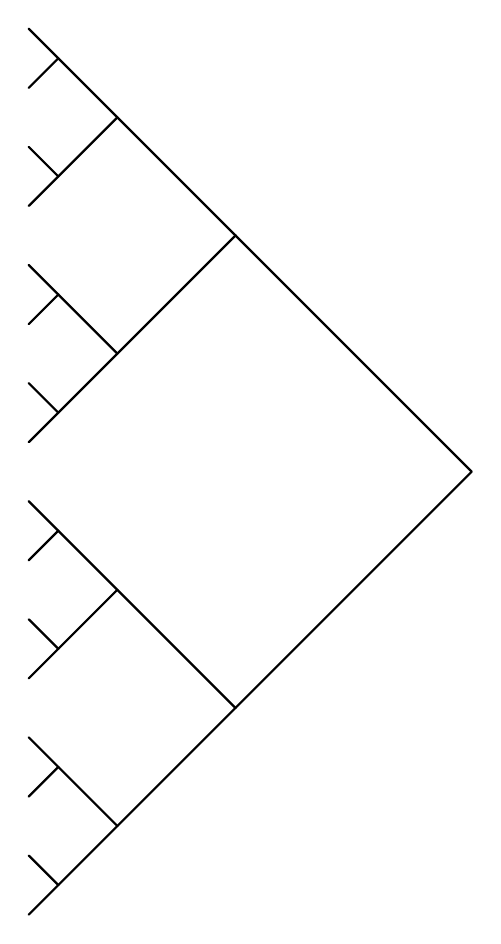
\begin{tikzpicture}[scale=3, line cap=round, line join=round]

% \fractaltree{depth}{x}{y}{length}
\newcommand{\fractaltree}[4]{%
  \ifnum #1>0
    % 以当前角度画一段主枝
    \begin{scope}
      \pgfmathsetmacro{\height}{-#4}
      \pgfmathsetmacro{\leftpos}{#4}
      \pgfmathsetmacro{\rightpos}{-#4}
      \draw[thick] (#2,#3) -- (\height,\rightpos); % 右枝
      \draw[thick] (#2,#3) -- (\height,\leftpos); % 左枝
      % 移到右枝末端,准备递归
      \begin{scope}[shift={(\height,\rightpos)}]
        % 计算下一层参数
        \pgfmathsetmacro{\nextlen}{#4*0.5}
        \pgfmathtruncatemacro{\nextd}{#1-1}
        % 递归左右子树
        \fractaltree{\nextd}{0}{0}{\nextlen}
      \end{scope}
      % 移到左枝末端,准备递归
      \begin{scope}[shift={(\height,\leftpos)}]
        % 计算下一层参数
        \pgfmathsetmacro{\nextlen}{#4*0.5}
        \pgfmathtruncatemacro{\nextd}{#1-1}
        % 递归左右子树
        \fractaltree{\nextd}{0}{0}{\nextlen}
      \end{scope}
    \end{scope}%
  \fi
}

% 从(0,0)开始,初始深度=4,初始长度=1
\fractaltree{4}{0}{0}{1}

\end{tikzpicture}
\end{document}
